\documentclass{standalone}
\usepackage{tikz}
\usepackage{graphicx}
\usetikzlibrary{positioning}

\begin{document}

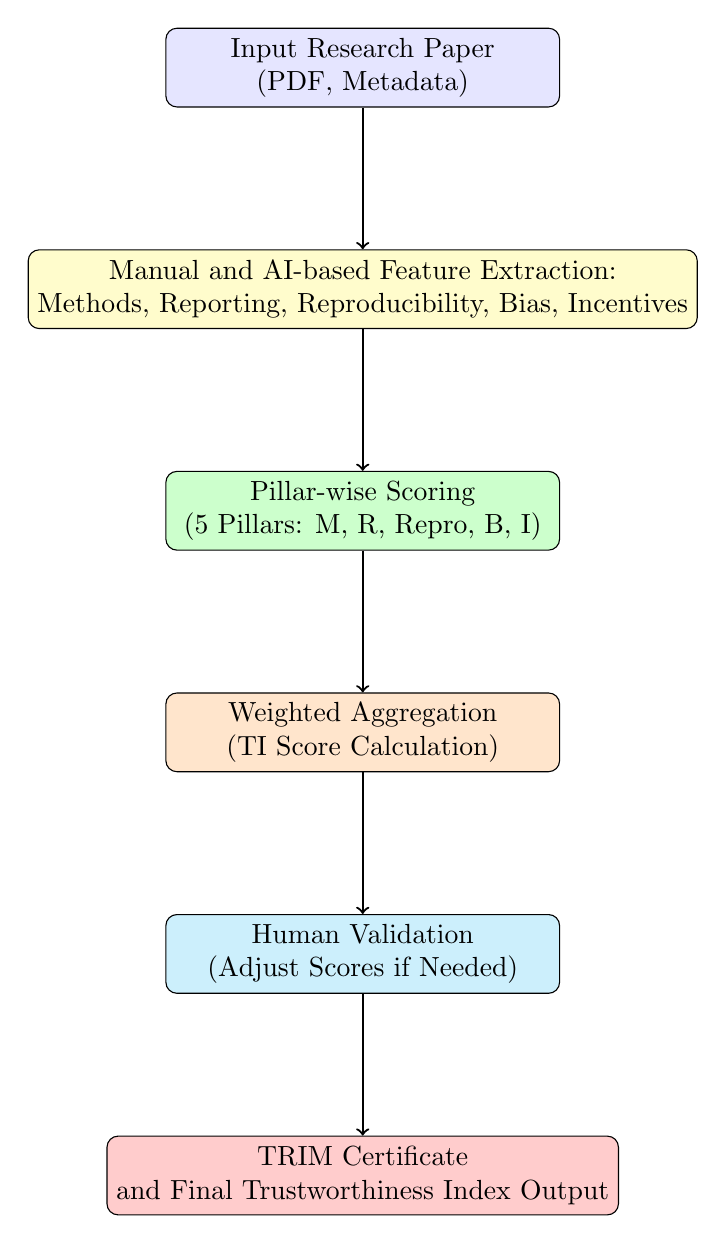
\begin{tikzpicture}[node distance=1.8cm and 2.5cm, every node/.style={align=center}]

% Main audit flow nodes
\node (input) [rectangle, draw, rounded corners, fill=blue!10, minimum width=5cm, minimum height=1cm] {Input Research Paper\\ (PDF, Metadata)};
\node (feature) [rectangle, draw, rounded corners, below=of input, fill=yellow!20, minimum width=5cm, minimum height=1cm] {Manual and AI-based Feature Extraction:\\ Methods, Reporting, Reproducibility, Bias, Incentives};
\node (pillar) [rectangle, draw, rounded corners, below=of feature, fill=green!20, minimum width=5cm, minimum height=1cm] {Pillar-wise Scoring\\ (5 Pillars: M, R, Repro, B, I)};
\node (weighting) [rectangle, draw, rounded corners, below=of pillar, fill=orange!20, minimum width=5cm, minimum height=1cm] {Weighted Aggregation\\ (TI Score Calculation)};
\node (audit) [rectangle, draw, rounded corners, below=of weighting, fill=cyan!20, minimum width=5cm, minimum height=1cm] {Human Validation\\ (Adjust Scores if Needed)};
\node (certificate) [rectangle, draw, rounded corners, below=of audit, fill=red!20, minimum width=5cm, minimum height=1cm] {TRIM Certificate\\ and Final Trustworthiness Index Output};

% Arrows
\draw[->, thick] (input) -- (feature);
\draw[->, thick] (feature) -- (pillar);
\draw[->, thick] (pillar) -- (weighting);
\draw[->, thick] (weighting) -- (audit);
\draw[->, thick] (audit) -- (certificate);

\end{tikzpicture}

\end{document}
